\documentclass[tikz,border=2pt]{standalone}

\usepackage{pgfplots}
\pgfplotsset{compat=1.18}

\begin{document}
	
	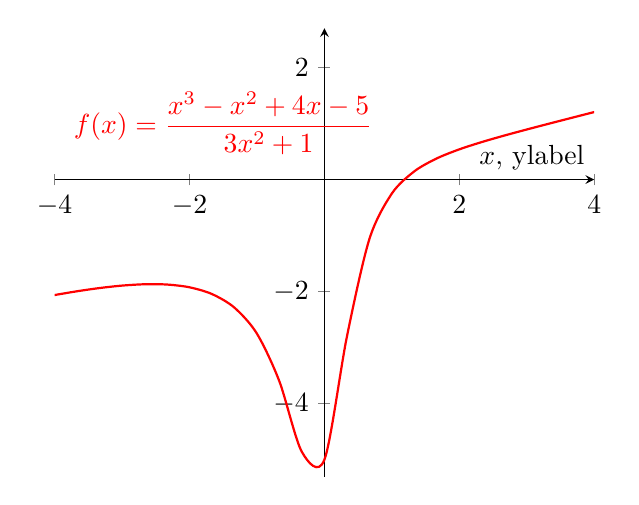
\begin{tikzpicture}
		\begin{axis}[
			xmin=-4,xmax=4,
			ymin=-5.3,ymax=2.7,
			axis lines=middle,
			xlabel=$x\text{,}$
			ylabel=$y\text{,}$
			legend style={yshift=120pt},
			legend style={xshift=-50pt},
			legend pos=south west,
			legend cell align={left}
			]
			\addplot[thick,red,domain=-4:4, smooth]{(x*x*x-x*x+4*x-5)/(3*x*x+1)};
			
			\node at (axis cs: -1.5,1){$\mathcolor{red}{\displaystyle f(x)=\frac{x^3-x^2+4x-5}{3x^2+1}}$};
		\end{axis}
	\end{tikzpicture}
	
\end{document}